\documentclass[xcolor=rgb]{beamer}

\usetheme{KSZK}

\usepackage{tikz}
\usepackage{smartdiagram}
\usepackage[english,hungarian]{babel}
   \usepackage{graphicx}
   \usepackage{amssymb}
   \usepackage{tikz}
   \title{Miért van szükség a nyelvtechnológiára?}
\author[\'Acs Judit]{\'Acs Judit}
  \institute{BME AUT}
  \date{KSZK40, 2016.~szeptember 23.}

\begin{document}
  
\begin{frame}
\titlepage 
\end{frame}

%TODO kell-e tartalomjegyzek?

\begin{frame}
    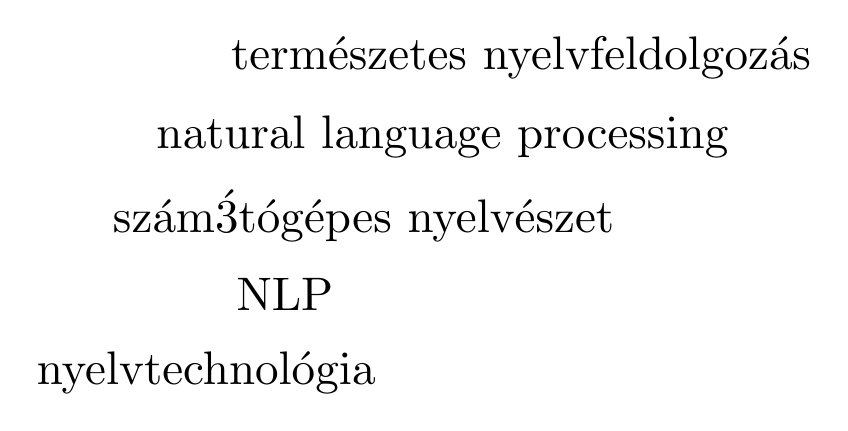
\begin{tikzpicture}
        \foreach[count=\i] \word in {nyelvtechnológia,NLP,számítógépes nyelvészet, natural language processing, természetes nyelvfeldolgozás} {
        \node[] at (\i,\i) {\scalebox{1.7}{\word}};
    };
  \end{tikzpicture}
\end{frame}

\begin{frame}
    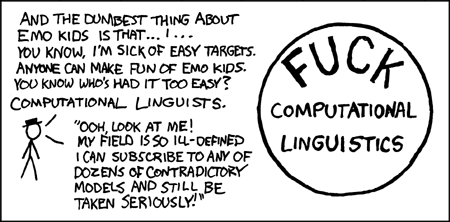
\includegraphics[width=\textwidth]{xkcd}

    \url{https://xkcd.com/114/}
\end{frame}

\begin{frame}{Interdiszciplináris}
    \begin{center}
        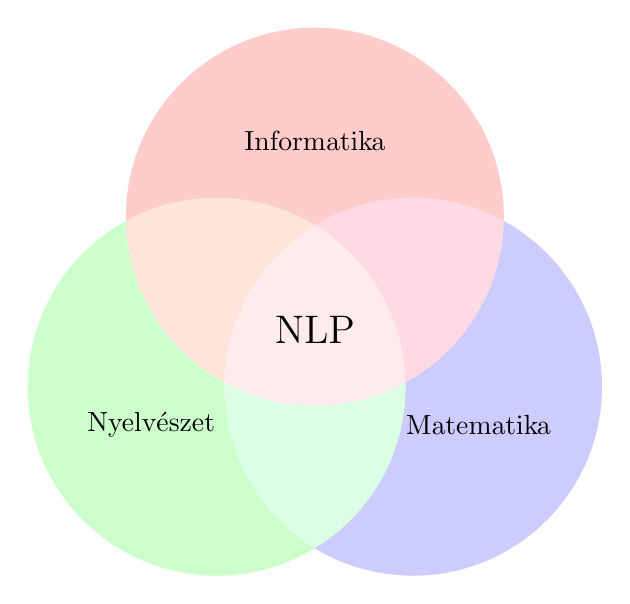
\begin{tikzpicture}[scale=1.2]
            \begin{scope}[blend group=soft light]
                \fill[red!20!white]   ( 90:1.2) circle (2);
                \fill[green!20!white] (210:1.2) circle (2);
                \fill[blue!20!white]  (330:1.2) circle (2);
            \end{scope}
            \node at ( 90:2)    {Informatika};
            \node at (210:2)    {Nyelvészet};
            \node at (330:2)    {Matematika};
            \node [font=\Large] {NLP};
        \end{tikzpicture}
    \end{center}
\end{frame}

\begin{frame}{Definíció?}
    \begin{itemize}
            \pause
        \item az input és/vagy az output természetes nyelv
            \pause
        \item formája sokféle lehet: írott, beszélt, jelnyelv, Braille stb.
    \end{itemize}
\end{frame}

\begin{frame}{Fordítás}
    \begin{itemize}
            \pause
        \item Fordítsuk le az alábbi mondatokat magyarra!
    \end{itemize}

    \begin{center}
        \Large 
    He went back to New York and left Mary behind. She was devastated.
    \end{center}
\end{frame}

\begin{frame}{Fordítás szavanként}
    He went back to New York and left Mary behind. She was devastated.

    \vspace*{.1cm}
    
    \visible<2->{Ő ment hát nak/nek Új York és van hátra Mary mögött.  Ő volt elpusztított.}

    \vspace*{.1cm}
    \begin{itemize}
        \item<3->  a \emph{back} szó kétértelmű (vissza, hát), \visible<8->{\textcolor{red}{word sense disambiguation}}
            \begin{itemize}
                \item<4-> \emph {left, devastated} is többértelműek
            \end{itemize}
        \item<5-> \emph{New York} egy tulajdonnév, \visible<9->{\textcolor{red}{named entity recognition}}
        \item<6-> \emph{She} kire vonatkozik? Angolul egyértelmű, magyarul nem, \visible<10->{\textcolor{red}{anaphora resolution}}
        \item<7-> \emph{went back} együtt fordítandó
        \item<7-> szórend, toldalékok
    \end{itemize}
\end{frame}

\begin{frame}{Google Translate}
    He went back to New York and left Mary behind. She was devastated.

    \vspace*{.3cm}
    \pause
    Visszament New York-i és a bal Mary mögött. Ő volt elpusztított.

    \begin{itemize}
            \pause
        \item \emph{New York-i} lett a \emph{to New York}ból,
            \pause
        \item \emph{left} rossz jelentését fordítja,
            \pause
        \item \emph{left behind}-ot szó szerint értelmezi?
            \pause
        \item a 2.~mondatról inkább ne beszéljünk.
    \end{itemize}
\end{frame}

\begin{frame}{NLP alapfeladatok}
    \begin{description}
            \pause
        \item[tokenizálás] szöveg kisebb egységekre bontása (mondat, szó).
            \pause
            \begin{itemize}
                \item \emph{New York-i} hány token?
                \item elválasztás
                \item dátumok kezelése stb.
            \end{itemize}
            \pause
        \item[szótövezés] toldalékok (képző, rag) eltávolítása. \emph{házaink - ház}
            \pause
            \begin{itemize}
                \item \emph{kályhák}, \emph{ettem}
            \end{itemize}
        \item[morfológiai elemzés]
            \pause
            \begin{itemize}
                \item \emph{zúzalékával}
            \end{itemize}
            \pause
        \item[névelemazonosítás] named entity recognition
            \pause
            \begin{itemize}
                \item \emph{Catholic} angolul, \emph{katolikus} magyarul
            \end{itemize}
    \end{description}
\end{frame}

\begin{frame}{NLP alapfeladatok II.}
    \pause
    \begin{description}
        \item[szófaji elemzés] part-of-speech tagging
    \pause
        \item[,,nyelvtani elemzés''] nyelvtani szerkezet feltárása. Különböző nyelvészeti elméletek különböző elemzéseket adnak.
        \pause
        \item[egyértelműsítés] word sense disambiguation
    \end{description}
\end{frame}

\begin{frame}{Magasabb szintű NLP feladatok}
    \begin{description}
            \pause
        \item[gépi fordítás] rule-based MT, statistical MT, neural MT
            \pause
        \item[koreferncia feloldás] mik utalnak ugyanarra az entitásra? \emph{New York -- Big Apple}
            \pause
        \item[szentiment analízis] vélemény, érzelem kinyerése
            \pause
        \item[kapcsolatkinyerés] relation extraction, ki kinek a rokona?
            \pause
        \item[kérdésmegválaszolás]
            \pause
        \item[szövegösszegzés] text summarization
            \pause
        \item[helyesírás-ellenőrzés]
    \end{description}
\end{frame}


\begin{frame}{Hogyan oldjuk meg ezeket a feladatokat?}
    \begin{enumerate}
            \pause
        \item Szabályalapú
            \pause
            \begin{itemize}
                \item kézzel írt szabályokat keresünk
                    \pause
                \item nagyon időigényes
                    \pause
                \item nem skálázódik
                    \pause
                \item jó pontosság, de milyen a fedés?
            \end{itemize}
                    \pause
        \item Gépi tanulás
            \pause
            \begin{itemize}
                \item felügyelt vs.~felügyeletlen
                    \pause
                \item a tanítóadat a legtöbb feladathoz nagyon költséges
                    \pause
                \item nem felügyelt módszerekhez sok adatunk van
                    \pause
                \item \emph{zaj!}
                    \pause
                \item itt pezseg jobban az élet
                    \pause
                \item deep learning
            \end{itemize}
    \end{enumerate}
\end{frame}

\begin{frame}{Adatok}
    \pause
    \begin{itemize}
        \item címkézett
            \pause
            \begin{itemize}
                \item névelemekre:
                    \pause
                \item New York - B-LOC E-LOC
                \item Google - ORG
                    \pause
                \item gold standard, silver standard
            \end{itemize}
            \pause
        \item címkézetlen
            \pause
            \begin{itemize}
                \item nyers szöveg
                \item kontextusból nyerhetünk információt
            \end{itemize}
            \pause
        \item rengeteg standard adat
            \pause
        \item de sose elég, 6000+ nyelv :(
    \end{itemize}
\end{frame}

\begin{frame}{Technológiai háttér}
    \begin{itemize}
            \pause
        \item Python, Java
            \pause
            \begin{itemize}
                \item NLTK (Natural Language Toolkit, Python)
                \item Stanford CoreNLP, Apache OpenNLP (Java)
            \end{itemize}
            \pause
        \item Linux (OSX)
            \pause
        \item gépi tanuláshoz: scikit-learn (Python), Weka (Java)
            \begin{itemize}
            \pause
                \item deep learning: tensorflow, theano, torch, keras stb.
            \end{itemize}
            \pause
         \item plain text, TSV, esetleg XML
             \pause
             \begin{itemize}
                 \item Linux CL toolokkal is elvégezhető sok egyszerű feladat (awk, sed)
             \end{itemize}
    \end{itemize}
\end{frame}

\begin{frame}{}

    \Large Hogyan készítenénk helyesírásellenőrzőt?

    \pause

    \vspace*{1cm}

    Hogyan sorolnánk fel az összes magyar szót?

    \pause

    \vspace*{1cm}

    Demo
\end{frame}

\begin{frame}{Köszönöm a figyelmet}
    \begin{center}
        judit@aut.bme.hu

        \vspace*{2cm}

            Demo: \url{https://gist.github.com/juditacs/4435129e6f79015ba98fba13f1736b84}

        \vspace*{2cm}
        Önlab, szakdolgozat, diplomaterv, TDK lehetőség
    \end{center}
\end{frame}

\end{document}
